\documentclass[11pt,preprint]{elsarticle}

\usepackage{lmodern}
%%%% My spacing
\usepackage{setspace}
\setstretch{1.2}
\DeclareMathSizes{12}{14}{10}{10}

% Wrap around which gives all figures included the [H] command, or places it "here". This can be tedious to code in Rmarkdown.
\usepackage{float}
\let\origfigure\figure
\let\endorigfigure\endfigure
\renewenvironment{figure}[1][2] {
    \expandafter\origfigure\expandafter[H]
} {
    \endorigfigure
}

\let\origtable\table
\let\endorigtable\endtable
\renewenvironment{table}[1][2] {
    \expandafter\origtable\expandafter[H]
} {
    \endorigtable
}


\usepackage{ifxetex,ifluatex}
\usepackage{fixltx2e} % provides \textsubscript
\ifnum 0\ifxetex 1\fi\ifluatex 1\fi=0 % if pdftex
  \usepackage[T1]{fontenc}
  \usepackage[utf8]{inputenc}
\else % if luatex or xelatex
  \ifxetex
    \usepackage{mathspec}
    \usepackage{xltxtra,xunicode}
  \else
    \usepackage{fontspec}
  \fi
  \defaultfontfeatures{Mapping=tex-text,Scale=MatchLowercase}
  \newcommand{\euro}{€}
\fi

\usepackage{amssymb, amsmath, amsthm, amsfonts}

\def\bibsection{\section*{References}} %%% Make "References" appear before bibliography


\usepackage[numbers]{natbib}

\usepackage{longtable}
\usepackage[margin=2.3cm,bottom=2cm,top=2.5cm, includefoot]{geometry}
\usepackage{fancyhdr}
\usepackage[bottom, hang, flushmargin]{footmisc}
\usepackage{graphicx}
\numberwithin{equation}{section}
\numberwithin{figure}{section}
\numberwithin{table}{section}
\setlength{\parindent}{0cm}
\setlength{\parskip}{1.3ex plus 0.5ex minus 0.3ex}
\usepackage{textcomp}
\renewcommand{\headrulewidth}{0.2pt}
\renewcommand{\footrulewidth}{0.3pt}

\usepackage{array}
\newcolumntype{x}[1]{>{\centering\arraybackslash\hspace{0pt}}p{#1}}

%%%%  Remove the "preprint submitted to" part. Don't worry about this either, it just looks better without it:
\makeatletter
\def\ps@pprintTitle{%
  \let\@oddhead\@empty
  \let\@evenhead\@empty
  \let\@oddfoot\@empty
  \let\@evenfoot\@oddfoot
}
\makeatother

 \def\tightlist{} % This allows for subbullets!

\usepackage{hyperref}
\hypersetup{breaklinks=true,
            bookmarks=true,
            colorlinks=true,
            citecolor=blue,
            urlcolor=blue,
            linkcolor=blue,
            pdfborder={0 0 0}}


% The following packages allow huxtable to work:
\usepackage{siunitx}
\usepackage{multirow}
\usepackage{hhline}
\usepackage{calc}
\usepackage{tabularx}
\usepackage{booktabs}
\usepackage{caption}


\newenvironment{columns}[1][]{}{}

\newenvironment{column}[1]{\begin{minipage}{#1}\ignorespaces}{%
\end{minipage}
\ifhmode\unskip\fi
\aftergroup\useignorespacesandallpars}

\def\useignorespacesandallpars#1\ignorespaces\fi{%
#1\fi\ignorespacesandallpars}

\makeatletter
\def\ignorespacesandallpars{%
  \@ifnextchar\par
    {\expandafter\ignorespacesandallpars\@gobble}%
    {}%
}
\makeatother


% definitions for citeproc citations
\NewDocumentCommand\citeproctext{}{}
\NewDocumentCommand\citeproc{mm}{%
\href{\#cite.\detokenize{#1}}{#2}\nocite{#1}}

\makeatletter
% allow citations to break across lines
\let\@cite@ofmt\@firstofone
% avoid brackets around text for \cite:
\def\@biblabel#1{}
\def\@cite#1#2{{#1\if@tempswa , #2\fi}}
\makeatother
\newlength{\cslhangindent}
\setlength{\cslhangindent}{1.5em}
\newlength{\csllabelwidth}
\setlength{\csllabelwidth}{3em}
\newenvironment{CSLReferences}[2] % #1 hanging-indent, #2 entry-spacing
{\begin{list}{}{%
	\setlength{\itemindent}{0pt}
	\setlength{\leftmargin}{0pt}
	\setlength{\parsep}{0pt}
	% turn on hanging indent if param 1 is 1
	\ifodd #1
	\setlength{\leftmargin}{\cslhangindent}
	\setlength{\itemindent}{-1\cslhangindent}
	\fi
	% set entry spacing
	\setlength{\itemsep}{#2\baselineskip}}}
{\end{list}}

\usepackage{calc}
\newcommand{\CSLBlock}[1]{\hfill\break\parbox[t]{\linewidth}{\strut\ignorespaces#1\strut}}
\newcommand{\CSLLeftMargin}[1]{\parbox[t]{\csllabelwidth}{\strut#1\strut}}
\newcommand{\CSLRightInline}[1]{\parbox[t]{\linewidth - \csllabelwidth}{\strut#1\strut}}
\newcommand{\CSLIndent}[1]{\hspace{\cslhangindent}#1}


\urlstyle{same}  % don't use monospace font for urls
\setlength{\parindent}{0pt}
\setlength{\parskip}{6pt plus 2pt minus 1pt}
\setlength{\emergencystretch}{3em}  % prevent overfull lines
\setcounter{secnumdepth}{5}

%%% Use protect on footnotes to avoid problems with footnotes in titles
\let\rmarkdownfootnote\footnote%
\def\footnote{\protect\rmarkdownfootnote}
\IfFileExists{upquote.sty}{\usepackage{upquote}}{}

%%% Include extra packages specified by user

%%% Hard setting column skips for reports - this ensures greater consistency and control over the length settings in the document.
%% page layout
%% paragraphs
\setlength{\baselineskip}{12pt plus 0pt minus 0pt}
\setlength{\parskip}{12pt plus 0pt minus 0pt}
\setlength{\parindent}{0pt plus 0pt minus 0pt}
%% floats
\setlength{\floatsep}{12pt plus 0 pt minus 0pt}
\setlength{\textfloatsep}{20pt plus 0pt minus 0pt}
\setlength{\intextsep}{14pt plus 0pt minus 0pt}
\setlength{\dbltextfloatsep}{20pt plus 0pt minus 0pt}
\setlength{\dblfloatsep}{14pt plus 0pt minus 0pt}
%% maths
\setlength{\abovedisplayskip}{12pt plus 0pt minus 0pt}
\setlength{\belowdisplayskip}{12pt plus 0pt minus 0pt}
%% lists
\setlength{\topsep}{10pt plus 0pt minus 0pt}
\setlength{\partopsep}{3pt plus 0pt minus 0pt}
\setlength{\itemsep}{5pt plus 0pt minus 0pt}
\setlength{\labelsep}{8mm plus 0mm minus 0mm}
\setlength{\parsep}{\the\parskip}
\setlength{\listparindent}{\the\parindent}
%% verbatim
\setlength{\fboxsep}{5pt plus 0pt minus 0pt}



\begin{document}



\begin{frontmatter}  %

\title{22894551 - Question 5 - An Apple a Day: Hack your Health}

% Set to FALSE if wanting to remove title (for submission)




\author[Add1]{Charisa Amorie Geyer}
\ead{22894551@sun.ac.za}





\address[Add1]{Stellenbosch University, Cape Town, South Africa}



\vspace{1cm}





\vspace{0.5cm}

\end{frontmatter}

\setcounter{footnote}{0}



%________________________
% Header and Footers
%%%%%%%%%%%%%%%%%%%%%%%%%%%%%%%%%
\pagestyle{fancy}
\chead{}
\rhead{}
\lfoot{}
\rfoot{\footnotesize Page \thepage}
\lhead{}
%\rfoot{\footnotesize Page \thepage } % "e.g. Page 2"
\cfoot{}

%\setlength\headheight{30pt}
%%%%%%%%%%%%%%%%%%%%%%%%%%%%%%%%%
%________________________

\headsep 35pt % So that header does not go over title




\section{Slide 1: Intro}\label{slide-1-intro}

Taking care of one's health is crucial because it impacts overall
well-being, including physical, mental, and emotional health, which in
turn affects daily life, productivity, and longevity. Good health allows
individuals to function optimally, cope with stress, and enjoy a higher
quality of life.

\section{Slide 2: What is BMR?}\label{slide-2-what-is-bmr}

Basal metabolic rate is the speed at which your body performs basic
metabolic functions. It the rate at which your body burns calories while
at rest, performing essential functions like breathing and circulation.
It represents the minimum number of calories needed to keep your body
functioning at a basic level. Essentially, it's the energy your body
uses just to stay alive when you're not actively doing anything.

\section{Slide 3: BMR threshold}\label{slide-3-bmr-threshold}

This threshold is calculated (differently for males and female). It
consists of a metric similar to BMI, where you take a transformed value
of your height, weight and activity levels to come to a factor. It is
sometimes calculated to see how many calories one should consume to
maintain your current weight.

\section{Slide 4: Determinants of
Health}\label{slide-4-determinants-of-health}

\begin{itemize}
\tightlist
\item
  Age -\textgreater{} older people have slower metabolisms
\item
  Muscle mass -\textgreater{} muscles burn calories
\item
  Body size -\textgreater{} having bigger organs requires more energy to
  keep you alive
\item
  Gender -\textgreater{} Men and Women have different bodily functions
  and hormone levels
\item
  Physical Activity -\textgreater{} strenous activity requires energy
\item
  Diet -\textgreater{} macronutrient intake makes a difference, more
  than just calories
\end{itemize}

\section{Silde 5: Who is healthy}\label{silde-5-who-is-healthy}

We can see here, that in this dataset of persons between 20 and 60, the
activity levels indicate an unexpected result. Further, stress levels
are also not following a clear trend. This is indicative of another
underlying fcactor determining the health.\\
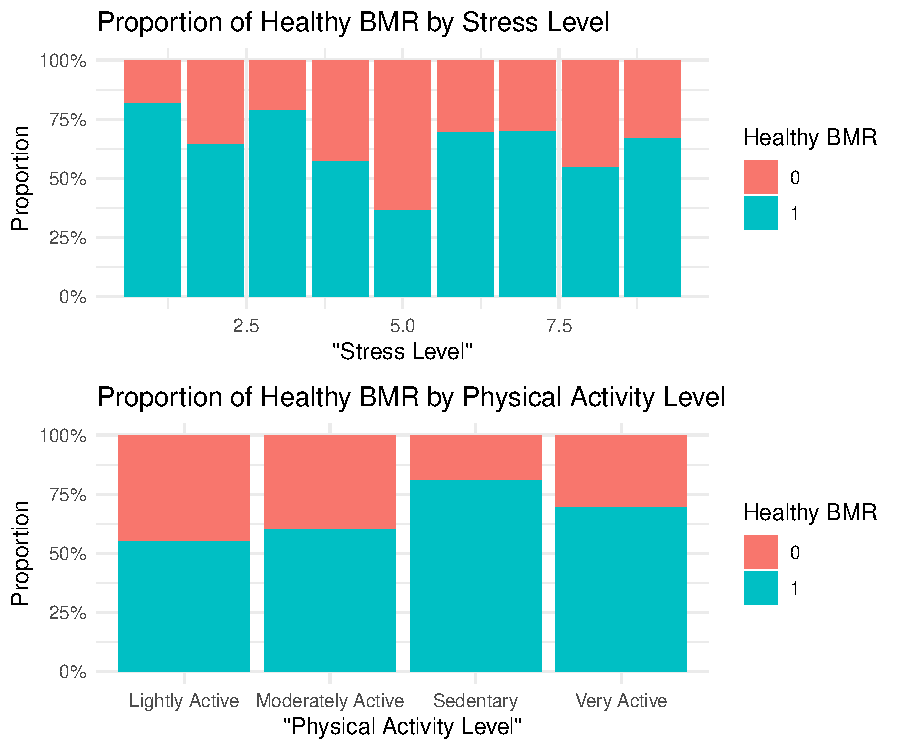
\includegraphics{Question5_files/figure-latex/unnamed-chunk-1-1.pdf}

\section{Slide 6: LPM results}\label{slide-6-lpm-results}

Men and women experience different effects. Remember that an LPM
measures effects relative to a basline category, which in this case is
low stress levels with excellent sleep and no activity. We can see
clearly (as clearly as LPM results can be), that excellent sleep is
always better, more moderate activity is acceptable and stress levels
have varying effects.

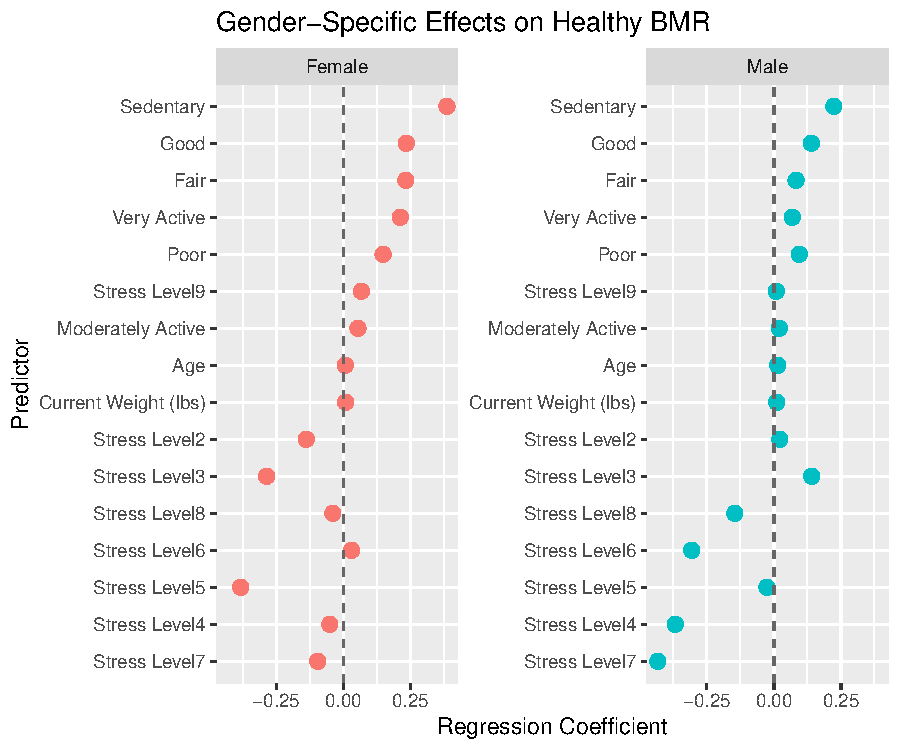
\includegraphics{Question5_files/figure-latex/unnamed-chunk-2-1.pdf}
\#\# What's next? * sleep more * exercise less * stop stressing about
your stress levels! This is of course a joke, and data can always be
wrangled in a way to fit a nrrative. So the lesson to learn is: DON'T
BELIEVE EVERYTHING THAT YOU SEE! Especially not if it comes from an
amateur analyst!

\subsection{Greetings}\label{greetings}

Thanks for listening and see you next time.

\bibliography{Tex/ref}





\end{document}
